\section{Reconstruction} % Seções são adicionadas para organizar sua apresentação em blocos discretos, todas as seções e subseções são automaticamente exibidas no índice como uma visão geral da apresentação, mas NÃO são exibidas como slides separados.
\begin{frame}{Signal Reconstruction}
    \begin{figure}
        \centering
        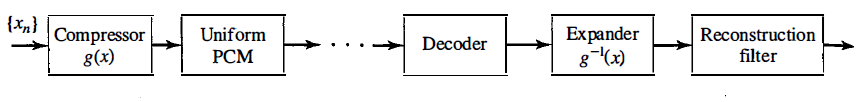
\includegraphics[width=0.7\linewidth]{img/non-unifor_PCM.png}
        % \caption{Diagrama de blocos do PCM}
        \label{fig:block_pcm}
    \end{figure}
       \begin{columns}

         \column{0.48\textwidth}  % First column
         Reconstruction Diagram
 \begin{figure}
        \centering
        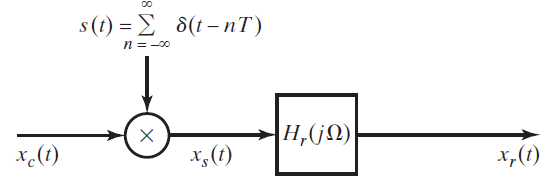
\includegraphics[width=1\linewidth]{img/reconstruction_3.png}
        % \caption{Diagrama de blocos do PCM}
        \label{fig:a-law}
    \end{figure}
    \column{0.48\textwidth}  % First column
Frequency Response and Reconstructed Signal
\begin{figure}
        \centering
        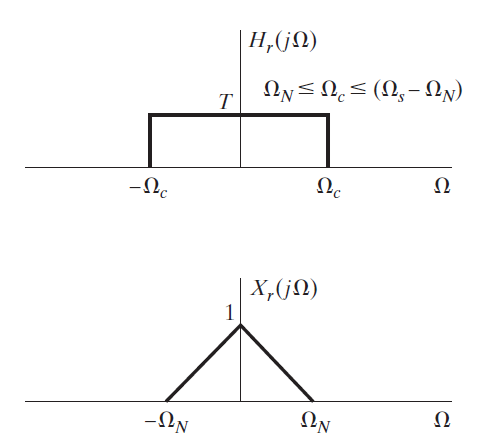
\includegraphics[width=.7\linewidth]{img/reconstruction_2.png}
        % \caption{Diagrama de blocos do PCM}
        \label{fig:a-law}
    \end{figure}
 
    \end{columns}
\end{frame}

%--------------------------------------------------------------------------------------------
\begin{frame}{Signal Reconstruction}
    \begin{figure}
        \centering
        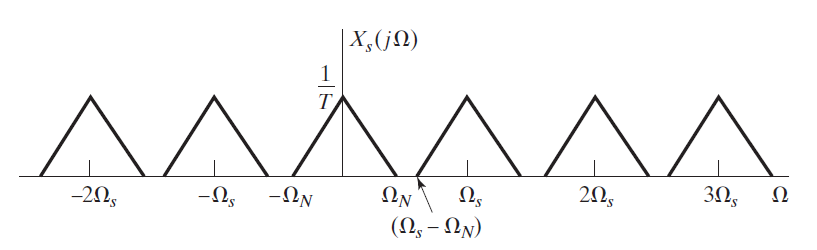
\includegraphics[width=0.7\linewidth]{img/reconstruction.png}
        % \caption{Diagrama de blocos do PCM}
        \label{fig:block_pcm}
    \end{figure}
\begin{figure}
        \centering
        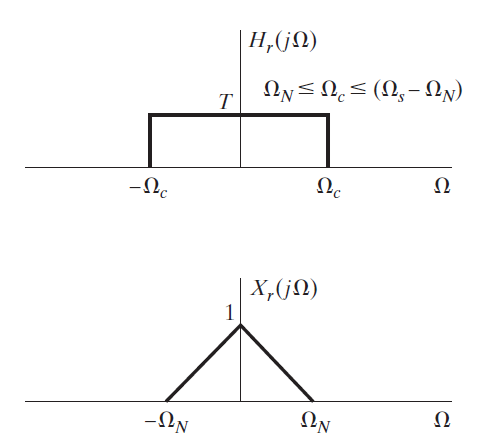
\includegraphics[width=.3\linewidth]{img/reconstruction_2.png}
        % \caption{Diagrama de blocos do PCM}
        \label{fig:a-law}
    \end{figure}
\end{frame}

% \begin{frame}{Referências}
%     \nocite{*}
%     \printbibliography[heading=none]
% \end{frame}